\section{Attention Mechanism}
\label{sec:nlp_attention}
The attention mechanism mimics the retrieval of a value $v_i$ for a query $q$ based on a key $k_i$ in database.
$$attn(q, k, v) = \sum_i sim(q,k_i)\times v_i$$
\begin{figure}[h]
	\centering
	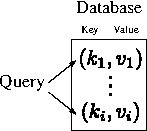
\includegraphics[scale=1.8]{./images/transformer/attention_database.pdf}
	\caption{The most similar key will be selected by measuring a \textbf{similarity} between a query and a key.}
\end{figure}

\begin{figure}[h]
	\centering
	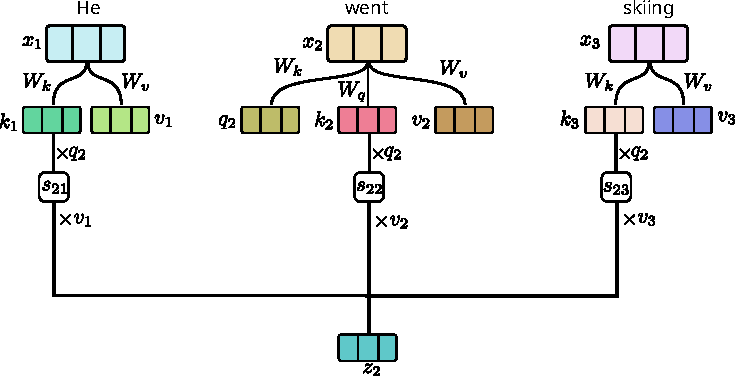
\includegraphics[scale=0.6]{./images/transformer/attention.pdf}
	\caption{The similarity $s_t$ is computed by a query and keys}
\end{figure}
There are several choices for a similarity function.
\begin{itemize}
	\item $q^Tk_i$: dot product.
	\item $\frac{q^Tk_i}{\sqrt{d}}$: scaled dot product $\to$ reduce the variance of the final attention weights. 
	\item $q^TWk_i$: general dot product.
	\item $w_q^Tq+ w_k^Tk_i$: additive similarity.
\end{itemize}
Finally, the \textbf{attention score} can be computed by using a softmax:
$$a_i = \frac{\exp(s_i)}{\sum_j \exp(s_j)}$$



### Key Idea:
The attention mechanism assigns **weights** (often called attention scores) to different parts of the input sequence, indicating how much each part contributes to the current output. In essence, the model "pays attention" to certain parts of the input more than others while processing each token in the sequence.

### Example of Attention Mechanism (Seq2Seq)
Let's use a machine translation task (English to French) as an example. Suppose we are translating the sentence "I am learning" into French. 

1. **Input**: Sequence of words in English: `[I, am, learning]`
2. **Output**: Sequence of words in French: `[Je, suis, en, train, d'apprendre]`

Instead of compressing all the input information into a fixed-size context vector (like in traditional encoder-decoder models), the attention mechanism allows the decoder to look at different parts of the input sentence at each step of the decoding process.

### Basic Structure of Attention

Given:
- An input sequence with tokens: \(\mathbf{x}_1, \mathbf{x}_2, ..., \mathbf{x}_n\)
- A decoder hidden state at time step \(t\): \(\mathbf{h}_t\)

The attention mechanism computes a **context vector** that represents a weighted combination of the encoder hidden states corresponding to the input tokens.

#### Steps in the Attention Mechanism:

1. **Step 1: Compute attention scores**  
   For each hidden state \(\mathbf{h}_t\) of the decoder, calculate the **alignment score** \(e_{t,i}\) between the decoder hidden state \(\mathbf{h}_t\) and each encoder hidden state \(\mathbf{s}_i\) (for input \(\mathbf{x}_i\)):

   \[
   e_{t,i} = \text{score}(\mathbf{h}_t, \mathbf{s}_i)
   \]

   The score function can vary, common ones include:
   - **Dot product**: \( e_{t,i} = \mathbf{h}_t^\top \mathbf{s}_i \)
   - **Additive** (Bahdanau Attention): \( e_{t,i} = \mathbf{v}_a^\top \tanh(\mathbf{W}_a \mathbf{h}_t + \mathbf{U}_a \mathbf{s}_i) \)

2. **Step 2: Compute attention weights**  
   Normalize the alignment scores using a softmax function to obtain the **attention weights**:

   \[
   \alpha_{t,i} = \frac{\exp(e_{t,i})}{\sum_{j=1}^{n} \exp(e_{t,j})}
   \]

   These weights \(\alpha_{t,i}\) tell us how much attention to pay to each input token when generating the output at time step \(t\).

3. **Step 3: Compute context vector**  
   Use the attention weights to compute a **context vector** \(\mathbf{c}_t\), which is a weighted sum of the encoder hidden states:

   \[
   \mathbf{c}_t = \sum_{i=1}^{n} \alpha_{t,i} \mathbf{s}_i
   \]

4. **Step 4: Generate output**  
   The context vector \(\mathbf{c}_t\) is then used along with the decoder hidden state \(\mathbf{h}_t\) to generate the final output (such as a translated word):

   \[
   \mathbf{o}_t = \text{generate}(\mathbf{h}_t, \mathbf{c}_t)
   \]

### Attention Matrix Visualization:
The attention weights \(\alpha_{t,i}\) can be represented as a matrix. Each row corresponds to a target word, and each column corresponds to a source word. The values in this matrix indicate how much each source word contributes to the target word at each step.

For example, if you're translating "I am learning" to French, the attention weights might look like this:

|             | I    | am   | learning |
|-------------|------|------|----------|
| Je          | 0.7  | 0.2  | 0.1      |
| suis        | 0.1  | 0.8  | 0.1      |
| en          | 0.05 | 0.15 | 0.8      |

This matrix shows that "Je" strongly attends to "I", "suis" attends mostly to "am", and "en" attends primarily to "learning".

### Types of Attention:

1. **Global Attention**: Attends to all input tokens at each step.
2. **Local Attention**: Attends to a subset of the input tokens (a window) at each step.

### Scaled Dot-Product Attention (Used in Transformers):
In Transformer models, the attention mechanism is slightly modified to include scaling:

\[
\text{Attention}(Q, K, V) = \text{softmax}\left(\frac{QK^\top}{\sqrt{d_k}}\right)V
\]

Where:
- \(Q\): Query matrix (derived from the decoder hidden state)
- \(K\): Key matrix (derived from the encoder hidden states)
- \(V\): Value matrix (also derived from encoder hidden states)
- \(d_k\): Dimension of the key vectors (used for scaling)

This version of attention allows for parallelization across different tokens and is the backbone of the Transformer architecture.

### Summary:
- **Attention** is a mechanism that helps the model focus on relevant parts of the input sequence at each decoding step.
- It assigns **weights** (attention scores) to different parts of the input and combines them into a **context vector**.
- The **context vector** is then used along with the decoder state to generate the output token.

The attention mechanism has dramatically improved the performance of models handling sequence-to-sequence tasks and is now used in modern architectures like the Transformer.




\section{Transformer}
\label{sec:nlp_transformer}
% The encoder's inputs first flow through a self-attention layer – a layer that helps the encoder look at other words in the input sentence as it encodes a specific word. 


\subsection{Self-Attention}
$$attn(Q,K,V) = softmax\bigg(\frac{Q^TK}{\sqrt{d_k}}\bigg)V$$

Here, $Q, K, V\in \mathbb{R}^{N\times d}$, $QK^T$'s time complexity is $O(N^2d)$. This quadratic cost is massive for long input-sequences such as documents to be summarized or character-level inputs.


\subsection{Masked attention}
The masked attention is often referred to cross-attention. This is just a self-attention in decoder.
$$\textrm{MA}(Q,K,V) = softmax\bigg(\frac{Q^TK+M}{\sqrt{d_k}}\bigg)V,$$
where $M$ is a matrix of 0 and $-\infty$. Note that $-\infty$ will make $exp$ term to be zero.

\subsection{Skip Connection}
This is a regularization technique.

\subsection{Positional Embedding}

\begin{figure}[t]
	\centering
	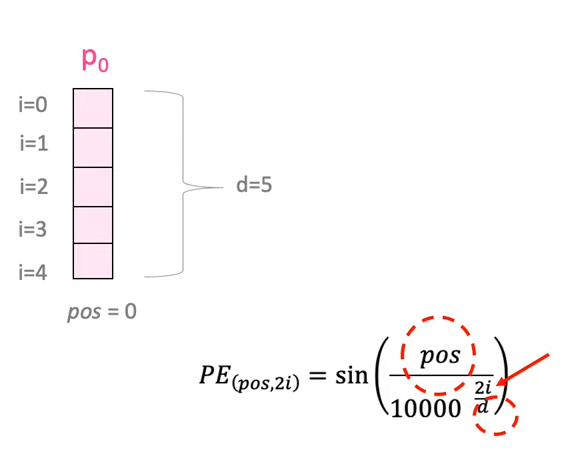
\includegraphics[scale=0.6]{./images/transformer/positional_1.png}
	\caption{Positional embedding.}
\end{figure}


\begin{lstlisting}[language=Python]
def position_encoding(seq_len: int, dim_model: int)->Tensor:
    pos = torch.arange(seq_len, dtype=torch.float).reshape(1, -1, 1)
    dim = torch.arange(dim_model, dtype=torch.float).reshape(1, 1, -1)
    phase = pos / (1e4 ** (dim // dim_model))
    return torch.where(dim.long() % 2 == 0, torch.sin(phase), torch.cos(phase))
\end{lstlisting}

\subsection{Encoder}

\subsection{Decoder}
The output of each step is fed to the bottom decoder in the next time step, and the decoders bubble up their decoding results just like the encoders did. And just like we did with the encoder inputs, we embed and add positional encoding to those decoder inputs to indicate the position of each word.

\begin{lstlisting}[language=Python]
def forward(self, tgt: Tensor, memory: Tensor) -> Tensor:
	seq_len, dimension = tgt.size(1), tgt.size(2)
	tgt += position_encoding(seq_len, dimension)
	for layer in self.layers:
		tgt = layer(tgt, memory)
	return torch.softmax(self.linear(tgt), dim=-1)
\end{lstlisting}


Self-attention (or intra-attention) is a mechanism where each token in an input sequence attends to every other token, including itself. It allows the model to capture dependencies within a sequence.

Given an input sequence $X = [x_1, x_2, \dots, x_n]$, where each $x_i$ is a word embedding (or token embedding), the self-attention mechanism follows these steps:

\subsection*{1. Create Query, Key, and Value vectors}

For each input token $x_i$, we create three vectors:
\begin{itemize}
	\item Query vector $Q_i$
	\item Key vector $K_i$
	\item Value vector $V_i$
\end{itemize}

These vectors are computed by multiplying the input embeddings with learned weight matrices:
\begin{itemize}
	\item Query: \( Q = XW_Q \)
	\item Key: \( K = XW_K \)
	\item Value: \( V = XW_V \)
\end{itemize}
Where \(W_Q\), \(W_K\), and \(W_V\) are the learned weight matrices.

Let's walk through an example of how self-attention works using a small sequence. Let's say we are given a sentence: ``She likes cats.''

Suppose the model has the following 3 word embeddings for "She", "likes", and "cats":
\[
X = [x_{\text{she}}, x_{\text{likes}}, x_{\text{cats}}]
\]

1. **Compute Queries, Keys, and Values:**
   Each word's embedding is transformed into a Query, Key, and Value using learned weight matrices \(W_Q\), \(W_K\), and \(W_V\):

   \[
   Q = XW_Q, \quad K = XW_K, \quad V = XW_V
   \]

   For simplicity, let's say the embeddings for each word are transformed into vectors:
   - **She**: \(Q_{\text{she}}, K_{\text{she}}, V_{\text{she}}\)
   - **Likes**: \(Q_{\text{likes}}, K_{\text{likes}}, V_{\text{likes}}\)
   - **Cats**: \(Q_{\text{cats}}, K_{\text{cats}}, V_{\text{cats}}\)

2. **Compute attention scores:**
   For each token, calculate attention scores with all other tokens. For instance, to compute how much "She" attends to "likes", we calculate \(Q_{\text{she}} \cdot K_{\text{likes}}\).

3. **Apply softmax to get weights:**
   After calculating the scores, apply the softmax function to get normalized attention weights. The attention weight tells how much attention "She" should pay to "likes" and "cats".

4. **Compute the weighted sum of values:**
   The output representation for "She" will be the weighted sum of the Value vectors for all tokens, with the weights being the attention scores.

### Scaled Dot-Product Self-Attention Equation

In general, the self-attention mechanism can be summarized by the following equation:

\[
\text{Attention}(Q, K, V) = \text{softmax}\left(\frac{Q K^\top}{\sqrt{d_k}}\right) V
\]

Where:
- \(Q\): Matrix of queries (from input embeddings).
- \(K\): Matrix of keys (from input embeddings).
- \(V\): Matrix of values (from input embeddings).
- \(d_k\): Dimensionality of the key vectors.

### Multi-Head Self-Attention:

In practice, self-attention is often used in a **multi-head** configuration, which means multiple self-attention mechanisms are applied in parallel, each with its own learned weights. The results of these parallel attention heads are concatenated and linearly transformed. This allows the model to focus on different parts of the sequence simultaneously.

Mathematically:
\[
\text{MultiHead}(Q, K, V) = \text{Concat}(\text{head}_1, \text{head}_2, \ldots, \text{head}_h)W^O
\]
Where:
- \(\text{head}_i = \text{Attention}(QW_Q^i, KW_K^i, VW_V^i)\)
- \(W_Q^i\), \(W_K^i\), \(W_V^i\) are learned weight matrices for each head.
- \(W^O\) is a weight matrix applied after concatenation.

### Intuition:

In a sentence like "The animal didn't cross the street because it was too tired", the word "it" could refer to "animal" or "street". Self-attention helps by allowing "it" to attend to the word "animal" based on the learned attention scores, enabling the model to resolve ambiguities and focus on the right words.

### Advantages of Self-Attention:

1. **Parallelization**: Unlike RNNs, which process tokens sequentially, self-attention can be computed in parallel for all tokens, making it highly efficient.
2. **Captures Long-Range Dependencies**: Self-attention can capture relationships between tokens that are far apart in the sequence.
3. **Scalability**: It works well with large sequences, as it allows each token to attend to all others.

Self-attention has become the foundation for modern models like the Transformer, BERT, GPT, and many others, significantly improving the ability to handle complex sequence tasks.


